% PREAMBULA DOKUMENTA
\documentclass[a4paper]{article}
\usepackage[slovene]{babel}
\usepackage[utf8]{inputenc}
\usepackage[T1]{fontenc}
\usepackage{graphicx}
\usepackage {lmodern}
\usepackage{amsfonts}
\usepackage{amsmath}
\usepackage{amssymb}
\usepackage{tikz}
\usepackage{mathtools}
\usepackage{wrapfig}
\usepackage{commath}
\usepackage{listings}
\usepackage{color}
\usepackage{caption}
\captionsetup[figure]{name=Slika}


\definecolor{codegreen}{rgb}{0,0.6,0}
\definecolor{codegray}{rgb}{0.5,0.5,0.5}
\definecolor{codepurple}{rgb}{0.58,0,0.82}
\definecolor{backcolour}{rgb}{0.95,0.95,0.92}

\lstdefinestyle{mystyle}{
    backgroundcolor=\color{backcolour},   
    commentstyle=\color{codegreen},
    keywordstyle=\color{magenta},
    numberstyle=\tiny\color{codegray},
    stringstyle=\color{codepurple},
    basicstyle=\footnotesize,
    breakatwhitespace=false,         
    breaklines=true,                 
    captionpos=b,                    
    keepspaces=true,                 
    numbers=left,                    
    numbersep=5pt,                  
    showspaces=false,                
    showstringspaces=false,
    showtabs=false,                  
    tabsize=2
}

\lstset{style=mystyle}
 


\begin{document}
\thispagestyle{empty}

\begin{figure}[t]
\begin{center} 

\includegraphics[width=6cm]{fmf.png}\\[4cm]
\end{center}
\end{figure}

\begin{center}
\Huge\textbf{Katzova središčnost in Googlov PageRank}\\[0.5cm]
\large\textsc{Poročilo projekta pri predmetu Finančni praktikum}\\[4cm]
\end{center}

\begin{flushleft}

\end{flushleft}
\vspace{\fill}
\begin{flushright}
Anamari Oštarijaš, Tina Ražić
\end{flushright}

\begin{flushleft}
Ljubljana, december 2018
\end{flushleft}

\newpage
\tableofcontents
\listoffigures

\newpage
\section{Opis projekta}
\hspace{4.8mm}Kompleksna omrežja lahko analiziramo z uporabo različnih kvantitetnih merjenj, imenujemo jih tudi mere središčnosti,  ki intuitivno zajamejo pomembnost določenih vozlišč. 
V projektu bova implementirali Googlov PageRank in Katzovo središčnost z uporabo potenčne metode. Na različnih grafih (tudi socialnih omrežjih) bova analizirali in primerjali, kako merjenji razvrstita vozlišča po pomembnosti. 

\section{Katzova središčnost}
\subsection{Matematično ozadje}


\hspace{4.8mm}Katzova središčnost izmeri vpliv igralca v omrežju tako, da upošteva direktne sosede igralca in vse druge igralce, ki so posredno povezani s tem igralcem preko njegovih direktnih sosedov. \\
Naj bo naše omrežje graf z $n$ vozlišči oziroma spletnimi stranmi. Naš graf predstavimo z matriko sosednosti A, torej element matrike $a_{ij}$ ima vrednost $1$, če je vozlišče $i$ povezano z vozliščem $j$, in $0$, če nista povezana. Katzovo središčnost $x_{i}$ vozlišča $i$ lahko zapišemo kot

$$x_{i} = \alpha\sum_{k}a_{i,k}x_{k} + \beta,$$
kjer sta $\alpha$ in $\beta$ konstanti. Konstanta $\beta$ je dana začetna središčnost vsakega vozlišča. Zapišimo zvezo v matrični formi:
$$x = \alpha Ax + \beta,$$
kjer je $\beta$ sedaj vektor, katerega komponente so enake dani konstanti. Sledi, da lahko vektor $x$ izračunamo kot
$$x =  (I - \alpha A)^{-1} \beta= \sum_{t=0}^{\infty} (\alpha A)^t \beta. $$

Vidimo, da je Katzova središčnost vozlišča določena z uteženimi potmi do ostalih vozlišč. Vsaka povezava v grafu dobi utež $\alpha$ in z $\alpha^{t}$ izračunamo težo povezave vozlišča z drugim vozliščem, pri čemer je $t$ število povezav med njima. Potence matrike A nam povejo, če je vozlišče povezano s drugimi indirektnimi vozlišči preko sosedov. Na primer, če je v matriki $A^{3}$ element $a_{2,5}  = 1,$ pomeni, da sta vozlišče $2$ in vozlišče $5$ povezana s tremi povezavami preko sosedov prve stopnje in sosedov druge stopnje.
Pri izbiri $\alpha$ moramo upoštevati omejitev 
$$0 < \alpha < \frac{1}{\abs{\lambda_{max}}},$$
saj pri $\alpha = \frac{1}{\abs{\lambda_{max}}}$ algoritem divergira. Za majhen $\alpha$ poti, ki imajo več kot eno povezavo do izbranega vozlišča, prispevajo zelo malo k središčnosti vozlišča. Na primer pri $\alpha = 0,$ izračun mere središčnosti sploh ne pride do izraza in imajo vsa vozlišča mero središčnosti $\beta.$  Pri večji izbrii $\alpha,$ pa se vpliv $\beta$ koeficienta manjša.


\subsection{Algoritem za Katzovo središčnost}
\begin{lstlisting}[language=Python]
def katz(G, max_num_of_steps, tolerance, alpha, beta, vector=None):
    '''Computes the Katz centrality for the nodes of the graph G.'''
    start = timer()
    A = nx.adjacency_matrix(G)
    diff = 1000
    k = 0
    ones = np.ones((A.shape[1], 1))
    if vector is None:
        vector = ones
    r = beta * vector
    while diff > tolerance and k < max_num_of_steps:
        # inner product of matrix A and vector r
        r, q = alpha*A.dot(r) + beta * ones, r
        diff = np.linalg.norm(q-r, ord=1)
        k += 1
    r = r/np.linalg.norm(r,ord = 2)
    print('process finished after {} iterations'.format(k))
    end = timer()
    # timing of the process
    print('time consumption: {} seconds'.format(end-start))
    return r
\end{lstlisting}


\section{Googlov PageRank}
\hspace{4.8mm}Nemogoče je definirati splošno mero pomembnosti, ki bi bila sprejemljiva za vse uporabnike iskalnika. Google uporablja pagerank za mero kakovosti spletnih strani. Temelji na predpostavki, da število linkov (povezav) do in iz strani daje informacijo o pomembnosti strani. \\
Popravi pomanjkljivost Katzove središčnosti, ki pravi, da je spletna stran pomembna, če je povezana s pomembno spletno stranjo. V resnici to ne drži, zato Googlov PageRank enakomerno porazdeli pomembnost spletne strani med vse povezave.
\subsection{Matematično ozadje}
Naj bodo vse spletne strani urejene s števili od $1$ do $n$ in naj bo $i$ neka spletna stran. Potem $O_i$ določa množico strani, s katerimi je $i$ povezana, tako da $i$ vsebuje link do strani v množici $O_i$ (\textit{outlink}). Število outlinkov označimo z $N_i = \|O_i\|$. Množica \textit{inlinkov}, označena z $I_i$, je množica strani, ki imajo outlink do $i$ (strani v $I_i$ vsebujejo linke do $i$).
Splošno, več ko ima stran $i$ inlinkov, pomembnejša je. \\ S takim sistemom bi bilo preprosto manipulirati (če bi nekdo želel, da njegovo spletno stran vidi čim več ljudi, bi ustvaril veliko število nepomembnih spletnih strani, ki bi vsebovale linke do njegove spletne strani). Da bi tako manipulacijo preprečili, definiramo rang vozlišča $i$ tako, da če ima visoko rangirana stran $j$ outlink do $i$, to doda pomembnosti $i$ na sledeč način: rang strani $i$ je utežena vsota rangov strani, ki imajo outlink do $i$. Obteženost  je taka, da je rang strani $j$ razdeljen enakomerno med njenimi outlinki. Z enačbo: $$r_i = \sum_{j \in I_1} \frac{r_j}{N_j}.$$ \\
Ta definicija je rekurzivna, zato pageranki ne morejo biti izračunani direktno. Uporabimo iteracijo. Najprej ugibamo začetni rangni vektor $r^0$. Potem iteriramo:
$$r_i^{(k+1)} = \sum_{j \in I_1} \frac{r_j^{(k)}}{N_j}.$$ \\
Raje zapišimo problem z matrikami. Naj bo $Q$ kvadratna matrika dimenzije $n$. Definiramo:
\[
Q_{ij} = 
\left \{
	\begin{array}{ll}
		1/N_j  &, \mbox{če obstaja link od j do i }  \\
		0 &, \mbox{sicer} 
	\end{array}
\right. \]
\\
Torej ima vrstica $i$ neničelne elemente na mestih inlinkov $i$. Podobno ima stolpec $j$ neničelne elemente enake $N_j$ na mestih  outlinkov $j$, vsota vseh elementov v stolpcu je enaka $1$. Definicija je ekvivalentna skalarnem produktu vrstice $i$ in vektorja $r$, ki vsebuje range vseh strani.\\
Enačbo sedaj lahko zapišemo v matrični obliki:
$$ \lambda r = Qr,     \qquad \lambda = 1,$$
Tako dobimo, da je $r$ lastni vektor matrike $Q$ z lastno vrednostjo $\lambda = 1$. Sedaj preprosto vidimo, da je iteracija ekvivalentna
$$r^{(k+1)} = Qr^{(k)},\qquad  k=0,1,… ,$$
kar je potenčna metoda za izračun lastnega vektorja.\\
\\ \textbf{Problem}: Ni jasno, da je pagerank dobro definiran, saj ne vemo ali obstaja lastna vrednost enaka 1. Pomagamo si s teorijo Markovske verige.\\
\\Obstaja interpretacija pageranka z naključnimi sprehodi. Predpostavimo, da uporabnik na spletni strani izbere naslednjo stran  med outlinki z enako verjetnostjo. Markovska veriga je slučajni proces v katerem je naslednje stanje določeno le s trenutnim stanjem, proces nima spomina. Prehodna matrika Markovske verige je $Q^T$.\\
Slučajni uporabnik nikoli ne sme obtičati. Z drugimi besedami, naš model slučajnega sprehoda ne sme imeti strani brez outlinkov (taka stran bi imela ničelni stolpec v $Q$). Torej je model prilagojen tako, da so ničelni stolpci nadomeščeni s konstantnimi vrednostmi na vseh mestih. To pomeni, da je enaka verjetnost, da pridemo na katero koli drugo spletno stran. \\ 
\\Definiramo vektorje: \\
\[
d_j = 
\left \{
	\begin{array}{ll}
		1  &, \mbox{če}\hspace{2mm} N_j = 0 \\
		0 &, \mbox{sicer} 
	\end{array}
\right. \]
za $j = 1, .., n$ in
$$e = [1 … 1] ^T \in \mathbb{R}^n.$$
Prilagojena matrika je definirana s $ P = Q + \frac{1}{n}ed^T$. 
S to prilagoditvijo je matrika $P$ desna stohastična matrika; vsi elementi so nenegativni in elementi vsakega stolpca se seštejejo v 1. \\
\\Desna stohastična matrika $P$ zadošča 
$$e^TP = e^T.$$ \\
Želimo definirati pagerank vektor kot enoličen lastni vektor matrike $P$ z lastno vrednostjo $1$:
$$Pr=r.$$ \\
Lastni vektor prehodne matrike je stacionarna verjetnostna porazdelitev Markovske verige. Element na mestu $i$ ($r_i$) je verjetnost, da po velikem številu korakov slučajni uporabnik pristane na strani $i$. Za zagotovitev enoličnosti mora biti matrika ireducibilna (slučajni uporabnik se lahko v nekem delu grafa zagozdi, v tem primeru ima matrika več lastnih vrednosti enakih $1$). \\ Edinstvenost največje lastne vrednosti ireducibilne, pozitivne, desne stohastične matrike je zagotovljena s \textit{Perron-Frobeniusovim izrekom}, največja singularna vrednost bo enaka $1$, pripadajoč lastni vektor je pozitiven in je edini lastni vektor, ki je nenegativen. \\
\\Zaradi velikosti spleta je matrika linkov $P$ reducibilna, torej pagerank lastni vektor ni dobro definiran. Da si zagotovimo ireducibilnost, umetno dodamo linke iz vsake spletne strani do vseh drugih. To lahko storimo, če vzamemo konveksno kombinacijo $P$ in matrike ranga 1:
$$A=\alpha P + (1-\alpha)\frac{1}{n}ee^T,$$
za nek $\alpha$, ki zadošča $0 \leq \alpha \leq 1$. Matrika $A$ je desna stohastična. Razlaga naključnega sprehoda dodatnega rang-1 izraza je, da bo uporabnik na vsakem časovnem koraku skočil na naključno stran z verjetnostjo $1- \alpha$.
Za konvergenco numeričnega algoritma za lastno vrednost je pomembno, da vemo, kako so s prilagoditvijo ranga-1 spremenjene lastne vrednosti.\\
\\ \textbf{Izrek:} \textit{Naj bodo lastne vrednosti desne stohastične matrike $P$ enake ${1, \lambda_2, \lambda_3, … , \lambda_n}$. Potem so lastne vrednosti $A=\alpha P + (1- \alpha) \frac{1}{n}ee^T$ enake ${1, \alpha \lambda_2, \alpha \lambda_3, … , \alpha \lambda_n}$.}\\
\\
Ta izrek nam pove, da tudi če ima $P$ več lastnih vrednosti enakih 1, kar je po navadi res, bo druga največja lastna vrednost matrike $A$ enaka $\alpha$. \\
Namesto prilagoditve lahko definiramo:
$$A = \alpha P + (1- \alpha)ve^T,$$
Kjer je $v$ nenegativen vektor z normo 1, ki je lahko izbran tako, da je iskanje pristransko do strani določene vrste. Zato ga včasih imenujemo \textit{personaliziran vektor}.

\subsection{Potenčna metoda}
Želimo rešiti problem lastne vrednosti:
$$Ar = r,$$
Kjer je $r$ nomaliziran $\|r\|_1=1$. Iskani lastni vektor označimo s $t_1$. \\
Prepostavimo, da imamo dan začetni približek $r{(0)}$. \\
\\
\textbf{Algoritem:} \\
\begin{center} za k = 1, 2, … do konvergence
	$$q^{(k)} = Ar^{(k-1)}$$ 
	$$r^{(k)} = q^{(k)}/ \|q^{(k)}\|_1$$ \\
\end{center}
Konvergenca je odvisna od porazdelitve lastnih vrednosti. Če je druga največja lastna vrednost blizu 1, bo iteracija zelo počasna. To na srečo ne velja za Google matriko. Vektor normaliziramo, da ne bi z iteracijami postali preveliki ali premajhni, posledično nereprezentativni s števili s plavajočo vejico. To v resnici ni potrebno, saj se v primeru desnih stohastičnih matrik temu izognemo.

\subsection{Algoritem za Googlov PageRank}
\begin{lstlisting}[language=Python]
def Qmatrix(matrika):
    '''za dano matriko sosednosti grafa vrne desno stohasticno matriko Q, kjer so nekateri stolpci se vedno nicelni'''
    #tabela vsot stolpcev matrike
    sums = np.sum(matrix, axis=0) 
    #vsak stolpec matrike delimo z njegovo vsoto, ce je vsota 0, vrne 0 namesto nan      
    return np.nan_to_num(matrix/sums)   

def dvector(matrika):
    '''za dano matriko sosednosti vrne transponiran vektor d, kjer d[j] = 1 ; ce #(outlinkov od j) = 0 in d[j] = 0 ; sicer'''
    Q = Qmatrix(matrix)             #izracunamo matriko Q
    sums = np.sum(matrix, axis=0)   #tabela vsot stolpcev matrike
    d_bool = (sums == 0)            #bool tabela, True ce je vsota stolpca enaka 0 in False sicer
    d = d_bool*1                    #False v 0 in True v 1
    return d

def evector(n):
    '''vrne vektor v iz samih enk velikosti n, kjer n = st. stolpcev v matriki'''
    return np.ones((n,1))    

def Pmatrix(matrix):
    '''vrne desno stohasticno matriko P'''
    n = matrix.shape[1]
    Q = Qmatrix(matrix)
    e = evector(n)
    d = dvector(matrix)
    return Q + 1/n*e.dot(d)

def Amatrix(matrix, alpha):
    '''vrne ireducibilno desno stohasticno matriko A, kjer je 0 <= alpha <= 1'''
    n = matrix.shape[1]
    e = evector(n)
    P = Pmatrix(matrix)
    return alpha*P + (1-alpha)*1/n*e.dot(e.transpose())

def pagerank2(matrix, max_num_of_steps, tolerance, alpha):
    '''vrne pagerank vektor matrike sosednosti grafa, 0 <= alpha <= 1'''
    start = timer()
    #desno stohasticna matrika dane matrike
    A = Amatrix(matrix, alpha)
    #ugibanje pagerank vektorja s prvim stolpcem matrike Q   
    r = A[:,0]  
    diff = 1000
    k = 0
    while diff > tolerance and k < max_num_of_steps:
        r, q = A.dot(r), r          #potencna metoda
        #razlika med prejsnjim in novim vekorjem r
        diff = np.linalg.norm(q-r, ord=1)   
        k+=1
    print('proces koncan po {} iteracijah'.format(k))
    end = timer()
    print('trajanje procesa: {} sekund'.format(end-start))  
    return r


\end{lstlisting}

\section{Analiza algoritmov}
\hspace{4.8mm}Analizirali sva učinkovitost algoritma na podlagi večih parametrov. Najbolj naju je zanimalo, kako izbira parametera $\alpha$, toleranca in število korakov vplivajo na hitrost algoritma in natančnost rezultata. \\
Uporabljali sva \textit{Facebook graf}, ki vsebuje $4039$ vozlišč in $88234$ povezav.
\begin{figure}[h]
\begin{center} 
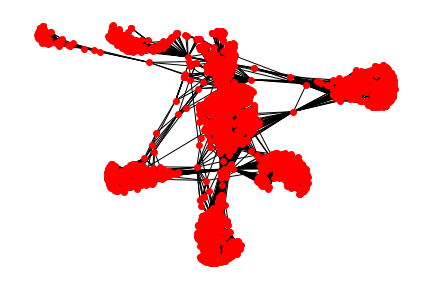
\includegraphics[width=6cm]{Facebook_graph.png}
\end{center}
\end{figure}

\subsection{Katzova središčnost}
\subsection{Izbira parametra $\beta$}
\hspace{4.8mm}Pri izračunu Katzove središčnosti uporabimo dve dani konstanti $\alpha$ in $\beta.$ Dana konstanta $\beta$ je začetna središčnost za vsa vozlišča, zato je vektor s konstantami $\beta$ naš začetni vektor pri potenčni metodi. Pogledali sva si primera, ko je $\beta =1$ in $\beta =50,$ pri fiksnem $\alpha = 0.003$. Spodaj b0omo videli, da je to dobra izbira $\alpha.$

\begin{lstlisting}[language=Python]
b1 = katz(G_fb, 10000000, 0.01, 0.003, 1)
b1
----------------------------------------------------------------
process finished after 15 iterations
time consumption: 0.4371460449999631 seconds
array([[0.02708885],
       [0.01358665],
       [0.01327441],
       ...,
       [0.01291167],
       [0.01299226],
       [0.01318997]])
\end{lstlisting}

\begin{lstlisting}[language=Python]
b2 = katz(G_fb, 10000000, 0.01, 0.003, 1000)
b2
----------------------------------------------------------------
process finished after 24 iterations
time consumption: 0.4746733580000182 seconds
array([[0.0270888 ],
       [0.01358663],
       [0.01327439],
       ...,
       [0.01291165],
       [0.01299224],
       [0.01318995]])
\end{lstlisting}

Opazimo, da parameter $\beta$ ne vpliva na rezultat algoritma, samo število iteracij se poveča. Poglejmo si graf zahtevnosti algoritma Katzove središčnosti v odvisnosti od $\beta.$

\begin{figure}[h]
\begin{center} 
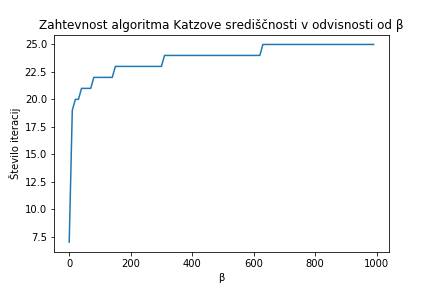
\includegraphics[width=9cm]{Katz_beta.png}
\caption[Zahtevnost algoritma Katzove središčnosti glede na $\beta$]{Graf števila iteracij pri danem $\beta$ izračunan na Facebook grafu.}
\end{center}
\end{figure}

Vidimo, da število iteracij naraste iz 15 na 25, medtem ko beta povečamo za 1000. Tudi trajanje algoritma se vseskozi giblje okoli 0.5 sekunde, torej parameter $\beta$ res nima znatnega vpliva na algoritem.

\subsection{Izbira parametra $\alpha$}
Pri preveliki izbiri $\alpha$ lahko algoritem divergira. Vemo, da mora biti $\alpha$ manjša od inverzne vrednosti največje lastne vrednosti. V našem primeru je največja lastna vrednost 162.37394233563828, torej za $\alpha$ velja omejitev $\alpha < 1/162.37 \doteq 0.00616.$ Poglejmo kaj se zgodi, če je $\alpha = 0.0062.$

\begin{lstlisting}[language=Python]
r1 = katz(G_fb, 10000000, 0.01, 0.0062, 1)
rank(r1)
----------------------------------------------------------------
process finished after 104436 iterations
time consumption: 213.18206373500004 seconds
RuntimeWarning: invalid value encountered in subtract

array([[   0],
       [2683],
       [2684],
       ...,
       [1352],
       [2018],
       [4038]], dtype=int64)
\end{lstlisting}

Naš proces se ustavi po dobrih 3 minutah in pojavi se napaka. Naj bo sedaj $\alpha = 0.0061.$

\begin{lstlisting}[language=Python]
r2 = katz(G_fb, 100000, 0.01, 0.0061, 1)
rank(r2)
----------------------------------------------------------------
process finished after 1056 iterations
time consumption: 1.1106130180000946 seconds
array([[3404],
       [1125],
       [ 577],
       ...,
       [  17],
       [  91],
       [ 361]], dtype=int64)
\end{lstlisting}

Proces se konča po 1056 iteracijah in v dobri 1 sekundi, kar je skoraj stokrat manj kot pri $\alpha = 0.0062$. Poglejmo, če se z manjšim $\alpha$, tudi število iteracij zmanjša. Najprej poskusimo z $\alpha = 0.003.$

\begin{lstlisting}[language=Python]
r3 = katz(G_fb, 10000000, 0.01, 0.003, 1)
rank(r3)
----------------------------------------------------------------
process finished after 15 iterations
time consumption: 0.2149773610003649 seconds
array([[3977],
       [1403],
       [ 807],
       ...,
       [  43],
       [ 175],
       [ 598]], dtype=int64)
\end{lstlisting}

Opazimo ogromen napredek. Sedaj algoritem potrebuje samo $15$ iteracij in približno $0.2$ sekundi.

Poglejmo si graf zahtevnosti algoritma Katzove središčnosti v odvisnosti od $\alpha.$

\begin{figure}[h]
\begin{center} 
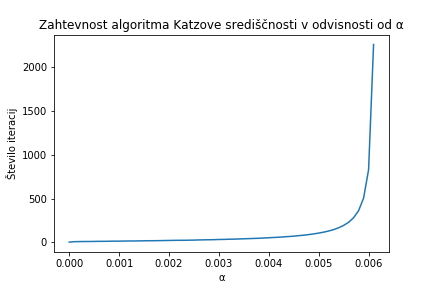
\includegraphics[width=9cm]{Katz_alpha.png}
\caption[Zahtevnost algoritma Katzove središčnosti glede na $\alpha$]{Graf števila iteracij pri danem $\alpha$ izračunan na Facebook grafu.}
\end{center}
\end{figure}

Vidimo, da število iteracij z večanjem konstante $\alpha$ zelo počasi narašča, ko pa se $\alpha$ približuje zgornji omejitvi, pa število iteracij eksponentno zraste.
Za primerjavo algoritma Katzove središčnosti z algoritmom PageRank bomo vzeli $\alpha = 0.003$, pri katerem algoritem potrebuje $15$ iteracij in $0.4$ sekunde ter $\beta = 1.$

\subsection{Googlov PageRank}
\subsubsection{Izbira parametra $\alpha$} 
\hspace{4.8mm}Vemo, da večji ko je $\alpha$, več podatkov o omrežju izgubimo. Torej želimo, da je ta parameter čim večji. \\
Poglejmo najprej kako velikost vpliva na čas izračuna pagerank vektorja. 

\begin{lstlisting}[language=Python]
M_fb = nx.adjacency_matrix(G_fb)
r_1 = pagerank2(M_fb,10000000,0.0000001, 0.98)
print(r_1)
----------------------------------------------------------------
proces koncan po 575 iteracijah
trajanje procesa: 11.7118154744594 sekund
[[  4.79508113e-03]
 [  2.17910466e-04]
 [  1.52316417e-04]
 ..., 
 [  6.77736016e-05]
 [  1.25649865e-04]
 [  2.72346363e-04]]
\end{lstlisting}

Izračun je bil končan po $575$ iteracijah in $11,71$ sekundah.

\begin{lstlisting}[language=Python]
r_2 = pagerank2(M_fb,10000000,0.0000001, 0.999)
print(r_2)
----------------------------------------------------------------
proces koncan po 4719 iteracijah
trajanje procesa: 61.73710875091092 sekund
[[  2.37207123e-03]
 [  1.15387662e-04]
 [  6.99886732e-05]
 ..., 
 [  2.37766591e-05]
 [  4.70770334e-05]
 [  1.04002744e-04]]
\end{lstlisting}
S povečanjem $\alpha$ smo povročili, da se je čas izračuna povečal na $61,74$ sekund, torej za več kot $5$ kratnik prejšnjega. 

\begin{lstlisting}[language=Python]
r_4 = pagerank2(M_fb,10000000,0.0000001, 0.9999)
print(r_4)
----------------------------------------------------------------
proces koncan po 8104 iteracijah
trajanje procesa: 105.30294071864228 sekund
[[  1.99799361e-03]
 [  9.77897213e-05]
 [  5.77554403e-05]
 ..., 
 [  1.28541957e-05]
 [  2.56615989e-05]
 [  5.75079410e-05]]
\end{lstlisting}

Večji ko je $\alpha$, več iteracij potrebujemo, da pridemo do željene tolerance. \\
Razlika med $r_1$ in $r_2$ v drugi normi je $0,00717920758147$, med $r_2$ in $r_4$ pa $0,00371765512728$, torej lahko z višjim $\alpha$ pričakujemo bolj natančne rezultate.  
\begin{figure}[h]
\begin{center} 
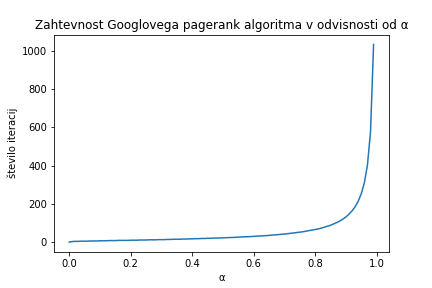
\includegraphics[width=9cm]{Pagerank_alpha.png}
\caption[Zahtevnost Googlovega pagerank algoritma glede na $\alpha$]{Graf števila iteracij pri danem $\alpha$ izračunan na Facebook grafu.}
\end{center}
\end{figure}

\newpage

\subsubsection{Izbira tolerance} 
\hspace{4.8mm}Očitno je, da višjo ko zastavimo toleranco, daljši bo postopek izračuna. Toleranco si izberemo sami in je odvisna od tega, kako natančen rezultat želimo. Tu sva za izračun sprotne tolerance v algoritmu izbrali prvo normo vektorja razlike med prejšnjim in trenutnim pagerank vektorjem ob določeni iteraciji, preprosto zaradi razloga, da je ta norma vedno večja ali enaka drugi normi vektorja. \\
\begin{figure}[h]
\begin{center} 
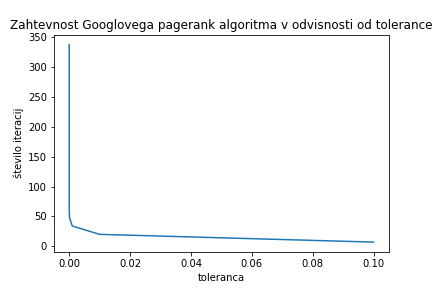
\includegraphics[width=9cm]{Pagerank_tolerance.png}
	\caption[Zahtevnost Googlovega pagerank algoritma glede na toleranco]{Graf števila iteracij pri $\alpha = 0.85$ glede na dano toleranco izračunan na Facebook grafu.}
\end{center}
\end{figure}


\section{Primerjava algoritmov}
Pri primerjavi algoritmov sva si pomagali z napisano funkcijo rank, ki nama vrne vektor rankiranih vrednosti, pri čemer ima vozlišče z najmanjšo središčnostjo najmanjši rank. Najprej sva najina algoritma preverili na majhnem grafu, potem pa še na večjih. 

\subsection{Majhen graf}
Majhen graf T ima 5 vozlišč in 5 usmerjenih povezav. Najina algoritma na grafu T vrneta isto razvrstitev pomembnosti vozlišč. 

\begin{figure}[h]
\begin{center} 
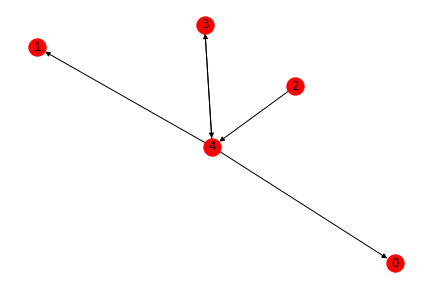
\includegraphics[width=9cm]{T_graph.png}
\caption[Razvrstitev pomembnosti vozlišč v majhnem grafu]{Razvrstitev pomembnosti vozlišč v majhnem grafu.}
\end{center}
\end{figure}

\subsection{Malo večji graf}
Za malo večji graf sva vzeli vgrajen graf Zachary's Karate Club v knjižnici networkx. Graf ima 34 vozlišč in 78 povezav. Najina algoritma samo 7 vozlišč enako rangirata. Do glaven razlike pride, ko pri Googlovem PageRank algoritmu pomembnost vsakega vozlišča razdelimo enakomerno med izhodne povezave, pri Katzovem algoritmu pa celotno pomembnost prenesemo na povezana vozlišča. 

\begin{figure}[h]
\begin{center} 
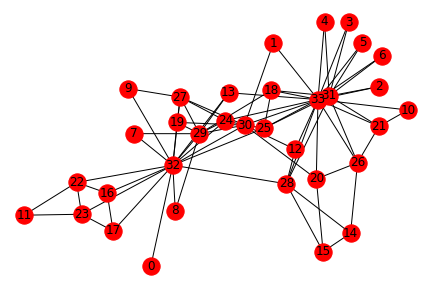
\includegraphics[width=6cm]{O_graph1.png}
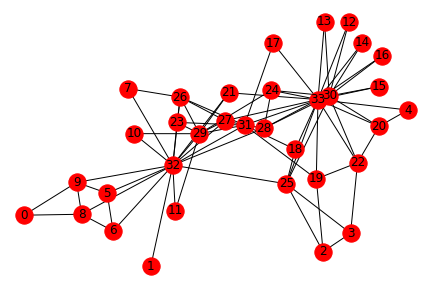
\includegraphics[width=6cm]{O_graph2.png}
\caption[Razvrstitev pomembnosti vozlišč v malo večjem grafu]{Razvrstitev pomembnosti vozlišč v malo večjem grafu z Googlovim PageRank algoritmom na levi in Katzovim algoritmom na desni.}
\end{center}
\end{figure}

Opazimo, da z obema algoritmoma na zunanjih vozliščih dobimo nižji rank, najpomembnejši vozlišči pa enako določita.

\subsection{Največji graf}
\end{document}
